\section{Results of DWBA post-form calculations}

\begin{figure}[t]
	\centering
	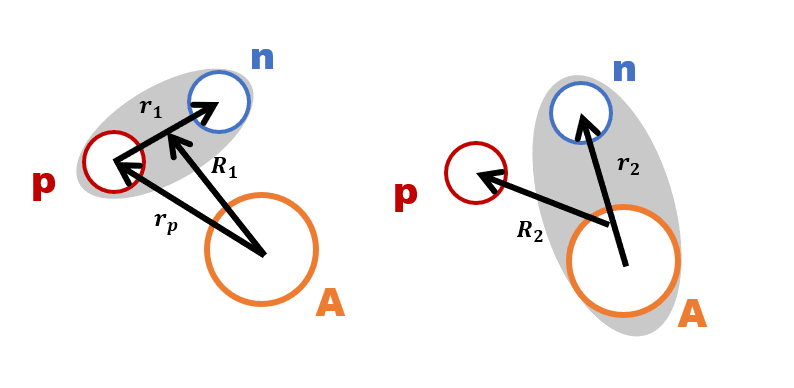
\includegraphics[width=0.80\textwidth]{transfer.png}
	\caption{Coordinates used in one neutron transfer reaction. }
	\label{fig:transfer}
\end{figure}
In a transfer reaction A(d,p)B showed in Fig. \ref{fig:transfer}, by introduction the auxiliary potential $U_f(R_2)$, the transfer T-matrix has a formula \cite{thompson2009nuclear}
\begin{equation}
	T_{post}=<\phi_{nA}\chi_{pB}^{(-)}\left|V_{np}(r_1)+U_{pA}(r_p)-U_f(R_2)\right|\Psi_1^+(\vec{r}_1,\vec{R}_1)>,
\end{equation}
where $\phi_{nA}$ and $\chi_{pB}$ are bound states wave-functions. 
Under DWBA approximation, it becomes
\begin{equation}\label{tpost}
	T_{post}^{DWBA}=<\phi_{nA}\chi_{pB}^{(-)}\left|V_{np}(r_1)+U_{pA}(r_p)-U_f(R_2)\right|\phi_{np}\chi_{dA}>.
\end{equation}
Besides that, we still need information for the auxiliary potential $U_f(R_2)$. 
It's usually chosen as $U_{pB}(R_2)$ fitted from elastic scattering.
We name $V_{np}(r_1)$ as binding potential and the rest two remnants.

Here are three different handling methods we used in our calculations.
\begin{enumerate}
\item Zero range approximation (ZRA): Remnants are neglected; $V_{np}(r_1)$ is considered as a local interaction with strength $D_0$.
	Correspondingly, the T-matrix becomes
	\begin{equation}
		T_{post}^{ZR-DWBA}=D_0<\phi_{nA}(R_1)\chi_{pB}^{(-)}| \chi_{dA}(R_1)>
	\end{equation}
	It now relies on $R_1$ only which simplifies calculation.
	\item First order DWBA without or with remnant: The former abandons the remnants but latter keeps, as well as the nonlocality of $V_{np}(r_1)$ is preserved in both.
\end{enumerate}

The results together with experimental data are presented in figures (need to be supplemented). 
We can see ZRA gives result deviates most from experiment because it applies the roughest approximation.
DWBA with or without remnants yield close results.
This makes sense because $U_{pA}$ and $U_{pB}$ are so similar that they almost cancel each other in Eq. \ref{tpost}.
But looking closer, we find the one with remnants is more contiguous to experiment.